% ******************************* PhD Thesis Template **************************
% Please have a look at the README.md file for info on how to use the template

\documentclass[a4paper,12pt,times,numbered,print,index]{Classes/PhDThesisPSnPDF}

% ******************************************************************************
% ******************************* Class Options ********************************
% *********************** See README for more details **************************
% ******************************************************************************

% `a4paper'(The University of Cambridge PhD thesis guidelines recommends a page
% size a4 - default option) or `a5paper': A5 Paper size is also allowed as per
% the Cambridge University Engineering Deparment guidelines for PhD thesis
%
% `11pt' or `12pt'(default): Font Size 10pt is NOT recommended by the University
% guidelines
%
% `oneside' or `twoside'(default): Printing double side (twoside) or single
% side.
%
% `print': Use `print' for print version with appropriate margins and page
% layout. Leaving the options field blank will activate Online version.
%
% `index': For index at the end of the thesis
%
% `draftclassic': For draft mode without loading any images (same as draft in book)
%
% `draft': Special draft mode with line numbers, images, and water mark with
% timestamp and custom text. Position of the text can also be modified.
%
% `abstract': To generate only the title page and abstract page with
% dissertation title and name, to submit to the Student Registry
%
% `chapter`: This option enables only the specified chapter and it's references
%  Useful for review and corrections.
%
% ************************* Custom Page Margins ********************************
%
% `custommargin`: Use `custommargin' in options to activate custom page margins,
% which can be defined in the preamble.tex. Custom margin will override
% print/online margin setup.
%
% *********************** Choosing the Fonts in Class Options ******************
%
% `times' : Times font with math support. (The Cambridge University guidelines
% recommend using times)
%
% `fourier': Utopia Font with Fourier Math font (Font has to be installed)
%            It's a free font.
%
% `customfont': Use `customfont' option in the document class and load the
% package in the preamble.tex
%
% default or leave empty: `Latin Modern' font will be loaded.
%
% ********************** Choosing the Bibliography style ***********************
%
% `authoryear': For author-year citation eg., Krishna (2013)
%
% `numbered': (Default Option) For numbered and sorted citation e.g., [1,5,2]
%
% `custombib': Define your own bibliography style in the `preamble.tex' file.
%              `\RequirePackage[square, sort, numbers, authoryear]{natbib}'.
%              This can be also used to load biblatex instead of natbib
%              (See Preamble)
%
% **************************** Choosing the Page Style *************************
%
% `default (leave empty)': For Page Numbers in Header (Left Even, Right Odd) and
% Chapter Name in Header (Right Even) and Section Name (Left Odd). Blank Footer.
%
% `PageStyleI': Chapter Name next & Page Number on Even Side (Left Even).
% Section Name & Page Number in Header on Odd Side (Right Odd). Footer is empty.
%
% `PageStyleII': Chapter Name on Even Side (Left Even) in Header. Section Number
% and Section Name in Header on Odd Side (Right Odd). Page numbering in footer
%set the page style to have page number at bottom, titles at top as set out by NUIG guidelines(http://www.nuigalway.ie/media/graduatestudies/files/university_guidelines_for_research_degree_programmes.pdf): Pages must be numbered consecutively, with page numbers located centrally at the bottom, and chapter headers at the top, of each page
% Uncomment to change page style
\pagestyle{PageStyleII}

% ********************************** Preamble **********************************
% Preamble: Contains packages and user-defined commands and settings
% ******************************************************************************
% ****************************** Custom Margin *********************************

% Add `custommargin' in the document class options to use this section
% Set {innerside margin / outerside margin / topmargin / bottom margin}  and
% other page dimensions
\ifsetCustomMargin
  \RequirePackage[left=40mm,right=30mm,top=35mm,bottom=30mm]{geometry}
  \setFancyHdr % To apply fancy header after geometry package is loaded
\fi

% Add spaces between paragraphs
%\setlength{\parskip}{0.5em}
% Ragged bottom avoids extra whitespaces between paragraphs
\raggedbottom
% To remove the excess top spacing for enumeration, list and description
%\usepackage{enumitem}
%\setlist[enumerate,itemize,description]{topsep=0em}

% *****************************************************************************
% ******************* Fonts (like different typewriter fonts etc.)*************

% Add `customfont' in the document class option to use this section

\ifsetCustomFont
  % Set your custom font here and use `customfont' in options. Leave empty to
  % load computer modern font (default LaTeX font).
  %\RequirePackage{helvet}

  % For use with XeLaTeX
  %  \setmainfont[
  %    Path              = ./libertine/opentype/,
  %    Extension         = .otf,
  %    UprightFont = LinLibertine_R,
  %    BoldFont = LinLibertine_RZ, % Linux Libertine O Regular Semibold
  %    ItalicFont = LinLibertine_RI,
  %    BoldItalicFont = LinLibertine_RZI, % Linux Libertine O Regular Semibold Italic
  %  ]
  %  {libertine}
  %  % load font from system font
  %  \newfontfamily\libertinesystemfont{Linux Libertine O}
\fi

% *****************************************************************************
% **************************** Custom Packages ********************************

% ************************* Algorithms and Pseudocode **************************

%\usepackage{algpseudocode}


% ********************Captions and Hyperreferencing / URL **********************

% Captions: This makes captions of figures use a boldfaced small font.
%\RequirePackage[small,bf]{caption}

\RequirePackage[labelsep=space,tableposition=top]{caption}
\renewcommand{\figurename}{Fig.} %to support older versions of captions.sty


% *************************** Graphics and figures *****************************

%\usepackage{rotating}
%\usepackage{wrapfig}

% Uncomment the following two lines to force Latex to place the figure.
% Use [H] when including graphics. Note 'H' instead of 'h'
%\usepackage{float}
%\restylefloat{figure}

% Subcaption package is also available in the sty folder you can use that by
% uncommenting the following line
% This is for people stuck with older versions of texlive
%\usepackage{sty/caption/subcaption}
%\usepackage{subcaption}

% ********************************** Tables ************************************
\usepackage{booktabs} % For professional looking tables
\usepackage{multirow}

%\usepackage{multicol}
%\usepackage{longtable}
%\usepackage{tabularx}


% *********************************** SI Units *********************************
\usepackage{siunitx} % use this package module for SI units


% ******************************* Line Spacing *********************************

% Choose linespacing as appropriate. Default is one-half line spacing as per the
% University guidelines

% \doublespacing
% \onehalfspacing
% \singlespacing


% ************************ Formatting / Footnote *******************************

% Don't break enumeration (etc.) across pages in an ugly manner (default 10000)
%\clubpenalty=500
%\widowpenalty=500

%\usepackage[perpage]{footmisc} %Range of footnote options


% *****************************************************************************
% *************************** Bibliography  and References ********************

%\usepackage{cleveref} %Referencing without need to explicitly state fig /table

% Add `custombib' in the document class option to use this section
\ifuseCustomBib
   \RequirePackage[square, sort, numbers, authoryear]{natbib} % CustomBib

% If you would like to use biblatex for your reference management, as opposed to the default `natbibpackage` pass the option `custombib` in the document class. Comment out the previous line to make sure you don't load the natbib package. Uncomment the following lines and specify the location of references.bib file

\RequirePackage[backend=biber, style=numeric-comp, citestyle=numeric, sorting=nty, natbib=true]{biblatex}

%\addbibresource{References/references} %Location of references.bib only for biblatex, Do not omit the .bib extension from the filename.
%\addbibresource{References/NonMendeleyReferences.bib} %Location of references.bib only for biblatex, Do not omit the .bib extension from the filename.
\fi

% changes the default name `Bibliography` -> `References'
\renewcommand{\bibname}{References}


% ******************************************************************************
% ************************* User Defined Commands ******************************
% ******************************************************************************

% *********** To change the name of Table of Contents / LOF and LOT ************

%\renewcommand{\contentsname}{My Table of Contents}
%\renewcommand{\listfigurename}{My List of Figures}
%\renewcommand{\listtablename}{My List of Tables}


% ********************** TOC depth and numbering depth *************************

\setcounter{secnumdepth}{2}
\setcounter{tocdepth}{2}


% ******************************* Nomenclature *********************************

% To change the name of the Nomenclature section, uncomment the following line

%\renewcommand{\nomname}{Symbols}


% ********************************* Appendix ***********************************

% The default value of both \appendixtocname and \appendixpagename is `Appendices'. These names can all be changed via:

%\renewcommand{\appendixtocname}{List of appendices}
%\renewcommand{\appendixname}{Appndx}

% *********************** Configure Draft Mode **********************************

% Uncomment to disable figures in `draft'
\setkeys{Gin}{draft=true}  % set draft to false to enable figures in `draft'

% These options are active only during the draft mode
% Default text is "Draft"
\SetDraftText{DRAFT}

% Default Watermark location is top. Location (top/bottom)
\SetDraftWMPosition{bottom}

% Draft Version - default is v1.0
\SetDraftVersion{v1.1}

% Draft Text grayscale value (should be between 0-black and 1-white)
% Default value is 0.75
%\SetDraftGrayScale{0.8}


% ******************************** Todo Notes **********************************
%% Uncomment the following lines to have todonotes.

\ifsetDraft
	\usepackage[colorinlistoftodos]{todonotes}
	
	\newcommand{\note}[1]{\todo[author=David,size=\small,inline,color=green!40]{#1}}
	
	\newcommand{\michaelnote}[1]{\todo[author=Michael,size=\small,inline,color=red!40]{#1}}
	
	\newcommand{\franknote}[1]{\todo[author=Frank,size=\small,inline,color=yellow!40]{#1}}
\else
	\newcommand{\note}[1]{}
	\newcommand{\listoftodos}{}
\fi

% Example todo: \mynote{Hey! I have a note}

% *****************************************************************************
% ******************* Better enumeration my MB*************
\usepackage{enumitem}


% ***********Define a new command to flag work as incomplete***********
\newcommand{\workinprogress}{\note{This part of the thesis is a work in progress, changes will be made and much of what you see are just ideas. High level feedback welcome.}}

% ***********Define a new command to flag work as incomplete***********
\newcommand{\placeholder}{\note{This work is mostly a placeholder and will be properly filled out in future. Much of this can just be ignored.}}

% ***********Define a new command to flag work as incomplete***********
\newcommand{\completedwork}{\note{I am happy that this section is complete}}

\newcommand{\michaelapproves}{\michaelnote{I have read over this section and don't think it needs any more work.}}

\newcommand{\frankapproves}{\franknote{I have read over this section and don't think it needs any more work.}}


\usepackage{amsmath}
%argmax used in HMM/DBN chapter
\DeclareMathOperator*{\argmax}{arg\,max}
\DeclareMathOperator*{\argmin}{arg\,min}


\usepackage{dcolumn}
\usepackage{booktabs}
\usepackage{tikz}
\usetikzlibrary{positioning,shapes,arrows}

\newcolumntype{M}[1]{D{.}{.}{1.#1}}

\usepackage{subfig}

\usepackage{verbatim}
\usepackage{bibentry}
\usepackage{natbib}
\nobibliography*




% ************************ Thesis Information & Meta-data **********************
% Thesis title and author information, refernce file for biblatex
% ************************ Thesis Information & Meta-data **********************
%% The title of the thesis
\title{A Multi-Agent System to aid the Automation of Search and Examination in Hazardous Environments}
%\texorpdfstring is used for PDF metadata. Usage:
%\texorpdfstring{LaTeX_Version}{PDF Version (non-latex)} eg.,
%\texorpdfstring{$sigma$}{sigma}

%% Subtitle (Optional)
\subtitle{}

%% The full name of the author
\author{David Smyth}

%% Department (eg. Department of Engineering, Maths, Physics)
\dept{College of Science and Engineering}

%% University and Crest
\university{National University of Ireland, Galway}
% Crest minimum should be 30mm.
%\crest{
\includegraphics[width=0.5\textwidth]{Figs/CollegeShields/src/NUI_Galway_BrandMark_B}}
\crest{
\includegraphics[width=0.5\textwidth]{Figs/CollegeShields/src/NUI_Galway_BrandMark_B.jpg}}
%% Use this crest, if you are using the college crest
%% Crest long miminum should be 65mm
%\crest{
\includegraphics[width=0.45\textwidth]{University_Crest_Long}}

%% College shield [optional] 
% Crest minimum should be 30mm.
%\collegeshield{
\includegraphics[width=0.2\textwidth]{CollegeShields/Kings}}


%% Supervisor (optional)
%% for multiple supervisors, append each supervisor with the \newline command
\supervisor{Prof. Michael G. Madden
\newline Dr. Frank G. Glavin}

%% Supervisor Role (optional) - Supervisor (default) or advisor
% \supervisorrole{\textbf{Supervisors: }}
%% if no title is desired:
% \supervisorrole{}

%% Supervisor line width: required to align supervisors
\supervisorlinewidth{0.5\textwidth}

%% Advisor (optional)
%% for multiple advisors, append each advisor with the \newline command
%\advisor{Dr. A. Advisor\newline
%Dr. B. Advisor}
     
%% Advisor Role (optional) - Advisor (default) or leave empty
% \advisorrole{Advisors: }
%% if no title is required
% \advisorrole{}

%% Advisor line width: required to align supervisors
%\advisorlinewidth{0.25\textwidth}


%% You can redefine the submission text:
% Default as per the University guidelines:
% ``This dissertation is submitted for the degree of''
%\renewcommand{\submissiontext}{change the default text here if needed}

%% Full title of the Degree
\degreetitle{Master of Science}

%% College affiliation (optional)
\college{National University of Ireland, Galway}

%% Submission date
% Default is set as {\monthname[\the\month]\space\the\year}
%\degreedate{September 2014} 

%% Meta information
\subject{LaTeX} \keywords{{LaTeX} {MSc. Thesis} {Engineering and Informatics} {National University of Ireland, Galway}}


% ***************************** Abstract Separate ******************************
% To printout only the titlepage and the abstract with the PhD title and the
% author name for submission to the Student Registry, use the `abstract' option in
% the document class.

\ifdefineAbstract
 \pagestyle{empty}
 \includeonly{Declaration/declaration, Abstract/abstract}
\fi

% ***************************** Chapter Mode ***********************************
% The chapter mode allows user to only print particular chapters with references
% Title, Contents, Frontmatter are disabled by default
% Useful option to review a particular chapter or to send it to supervisior.
% To use choose `chapter' option in the document class

\ifdefineChapter
 \includeonly{Chapter3/chapter3}
\fi

% ******************************** Front Matter ********************************
\begin{document}



\frontmatter

\maketitle

%% ******************************* Thesis Dedidcation ********************************

\begin{dedication} 

\end{dedication}


%% ******************************* Thesis Declaration ***************************

\begin{declaration}

I declare that this thesis has been composed by me and I have not obtained a degree from the National University of Ireland, Galway, or elsewhere, on this work previously.

% Author and date will be inserted automatically from thesis.tex \author \degreedate

\end{declaration}


%% ************************** Thesis Acknowledgements **************************

\begin{acknowledgements}      

\end{acknowledgements}

% ************************** Thesis Abstract *****************************
% Use `abstract' as an option in the document class to print only the titlepage and the abstract.

\nomenclature[]{AI}{Artificial Intelligence}

\begin{abstract}
% maybe should modify this to include some notes about how multi-agent systems are becoming more ubiquitous in society and that they naturally solve many research problems.

\workinprogress{}

Systems utilitising autonomous agents are becoming increasingly pervasive in today's society, garnering commercial interest and research funding in a variety of domains ranging from home automation to undersea exploration. This has stemmed from a resurgence in interest in Aritifical Intelligence over the last number of years. Globally, we are starting to move towards an age of automation through physical and software systems that exhibit redundancy, modularity and robustness. Research into how to induce intelligent decentralised behaviour in such systems will be key to their development.\par
Autonomous systems that can be operated remotely are highly suitable to disaster scene management, due to their highly dangerous and uncertain nature. This thesis outlines the design and implementation of a team of autonomous robots that implement a multi-phase disaster scene management plan.
%the goal of which is to solve a real-world problem in the domain of disaster scene management. 
The problem domain involves robotic aerial vehicles that have sensors and actuators to interact with their environment. Our framework is described abstractly and can be used with different physical agents, with few restrictions on the capabilities and specification of the agents.\par

First, the design and development of a purpose-built high-fidelity simulation environment using a game engine is outlined. This simulation environment has been used extensively in the research project, ROCSAFE, that motivated the work in this thesis. The ROCSAFE project is discussed in section \ref{sec:ROCSAFEBG}. The simulation environment has helped to address the problem of generating data to carrying out training, testing and validation of systems related to the management of scenarios that are perilous in nature. It has proved a valuable tool for prototyping the work that has been done as part of this thesis.

We then discuss the problem of developing an autonomous system to aid the management of a disaster scene. The problem can be broken down into two key sub-problems. The first is a surveying problem, whereby a swarm of aerial vehicles need to use sensors to record data at each point in a discretised region defined by a bounding polygon. This is a standard early phase of a forensic examination of a crime scene and the data gathered from this survey can be used to guide strategies used during subsequent phases of the disaster management process. %Examples of how this information can be used are presented, such as using structure-from-motion to create a textured point cloud that can then be used to plan a safe path for forensic evidence recovery by a ground vehicle.
\par

The second is a search problem, where multiple agents are used to pinpoint the location of a target, or multiple targets, in a bounding region. The term "target" is used to mean anything that can be sensed by the agents, for example a source of radioactive material. It is assumed that agents are fitted with sensors and actuators and can move around the bounding region freely. Sensor readings are assumed to have some inherent noise, and a probabilistic approach is presented which takes this fact into account. Analysis of the framework is presented to give insight into how it can be used to formulate search control strategies that optimise some realistic objectives. Constraints present in the real world are enforced, such as limited communication between agents. The results of using the custom-built simulation environment to run the system are presented.\par



%the developed system is tested using a purpose built simulation environment, which is intended to be a high-fidelity representation of a forensic examination scenario and results are presented.\par

%Results show that the system developed ...
%\break
%List of things that need to be changed
%\begin{enumerate}
%    \item Sometimes mistakenly used 'multinomial', change where appropriate
%    \item Change small n to big N when referring to grid
%    \item discuss how varying height can be incorporated to sensor model
%    \item Check references are correct and fix formatting
%    \item Sometimes use "source" when should be "target"
%\end{enumerate}

\end{abstract}

%include summary of Contents

% *********************** Adding TOC and List of Figures ***********************

\tableofcontents
% ******************************* Thesis Declaration ***************************

\begin{declaration}

I declare that this thesis has been composed by me and I have not obtained a degree from the National University of Ireland, Galway, or elsewhere, on this work previously.

% Author and date will be inserted automatically from thesis.tex \author \degreedate

\end{declaration}



\listoffigures

\listoftables

% \printnomenclature[space] space can be set as 2em between symbol and description
%\printnomenclature[3em]

\printnomenclature

% ******************************** Main Matter *********************************
\mainmatter

%!TEX root = ../thesis.tex
%*******************************************************************************
%*********************************** First Chapter *****************************
%*******************************************************************************


%*******************************************************************************
%*********************************** Nomenclature *****************************
%*******************************************************************************

\nomenclature[A]{AI}{Artificial Intelligence}
%introduce some nomenclature
%\nomenclature[]{Percept}{A percept is an interpreted reading of the state of the environment, taken by the agent's sensor}
%\nomenclature[]{Action}{An action is ...}
%\nomenclature[]{State}{A state is ...}
%\nomenclature[]{Utility function}{A utility function is a function that maps a sequence of states to a real number. It is used to give a value to the outcome of actions. }
%\nomenclature[Y]{Performance Measure}{A performance measure is }
\nomenclature[A]{MAS}{Multi-Agent System}
\nomenclature[A]{DBN}{Dynamic Bayesian Network}
\nomenclature[A]{BN}{Bayesian Network}
\nomenclature[A]{CPD}{Conditional Probability Distribution}
\nomenclature[A]{2TDBN}{2 Time Slice Dynamic Bayesian Network}
\nomenclature[A]{CPD}{Conditional Probability Distribution}
\nomenclature[A]{HMM}{Hidden Markov Model}
\nomenclature[A]{MLE}{Maximum Likelihood Estimate}
\nomenclature[A]{SPRT}{Sequential Probability Ratio Test}
\nomenclature[A]{FPR}{False Positive Rate}
\nomenclature[A]{FNR}{False Negative Rate}
\nomenclature[A]{UUV}{Unmanned Underwater Vehicle}
\nomenclature[A]{UE4}{Unreal Engine 4}
\nomenclature[A]{RAV}{Robotic Aerial Vehicle}
\nomenclature[A]{GPS}{Global Positioning System}
\nomenclature[A]{WGS84}{World Geodetic System 1984}
\nomenclature[A]{VRP}{Vehicle Routing Problem}
\nomenclature[A]{TSP}{Travelling Salesman Problem}
\nomenclature[A]{CBRNe}{Chemical, Biological, Radiological, Nuclear, explosive}
\nomenclature[A]{ROCSAFE}{Remotely Operated CBRNE Scene Assessment and Forensic Examination}
%*******************************************************************************
%*********************************** Nomenclature *****************************
%*******************************************************************************






\chapter{Introduction}\label{chapter:introduction}  %Title of the First Chapter

\placeholder{}

\ifpdf
    \graphicspath{{Chapter1/Figs/Raster/}{Chapter1/Figs/PDF/}{Chapter1/Figs/}}
\else
    \graphicspath{{Chapter1/Figs/Vector/}{Chapter1/Figs/}}
\fi


%********************************** %First Section  **************************************
\section{Motivation and Scope} %Section - 1.1 
\nomenclature[F]{CBRNE}{Chemical, Biological, Radiological, Nuclear, explosive}

Technologies based on systems of intelligent agents have received an increasing amount of interest in both research an industry in recent years. Mobile robotics applications such as Simultaneous Localization and Mapping (SLAM) and target detection and tracking have received substantial interest in particular, with a focus on the multi-robot setting\cite{Saeedi2016Multiple-RobotReview}, \cite{Robin2016Multi-robotSurvey}. This is due to factors such as increased computing power, decreasing lightweight sensor costs, more accurate models of robot environments and improved simulation technologies. Application domains have naturally gravitated towards problems that would pose hazards to physical human presence. This work has been funded and motivated by a EU Horizon 2020 research project called ROCSAFE (Remotely Operated Chemical, Biological, Radiological, Nuclear(CBRN) Scene Assessment and Forensic Examination)\cite{rocsafeNUIG}. The goal of the project is to fundamentally change how CBRNe scenes are assessed by ensuring the safety of crime scene investigators. The project uses autonomous robots to reduce the need for them to enter high-risk areas when their job requires the determination of threats and gathering of  forensic evidence.\par

The scope of this thesis lies in developing agents in the realm of mobile robotics, in order to carry out tasks that are of value in scenarios that would present dangers to humans. A system of heterogeneous aerial vehicles is considered, with sensing capabilities as well as high-level collision avoidance and navigation capabilities. The focus is primarily on designing software that implements strategies to efficiently carry out area surveillance and target localization, independent of the hardware on board the aerial vehicles. Realistic constraints such as operational speeds and battery capacity are considered. The use of high-fidelity 3-D simulation environments has also been investigated, due to the highly complex nature of hazardous real-world scenarios that require monitoring. This has complemented much of the research that has been carried out in parallel in the ROCSAFE research project, for example image processing modules.\par



\section{Research Questions}\label{sec:ResearchQuestions} %Section - 1.3 
We identified two main research questions to be investigated for this thesis. They are as follows:
\begin{enumerate}

    \item Can an agent-based software system be developed to run on a system of heterogeneous autonomous aerial vehicles to aid the tasks of scene surveying and target localisation in a hazardous environment? 
    
    \item Can a high-fidelity simulation environment be designed to simulate a hazardous environment, which can generate realistic data to aid the process of prototyping and developing AI systems to be deployed in the real world?
    
\end{enumerate}

Both research questions were derived from the aims of the ROCSAFE project. \href{https://www.nuigalway.ie/rocsafe/research/}{Deliverable 2.3}\footnote{\href {https://www.nuigalway.ie/rocsafe/research/}{https://www.nuigalway.ie/rocsafe/research/}} of the project provides a gap analysis in the management of the forensic phase of a crime scene. 
%the document is based on....
Among the topics that were addressed were
\begin{itemize}
    \item Scene Assessment: The document identifies a gap in scene assessment capabilities at the time of publication: 
"\textit{Currently only limited means are available for remote scene assessment. These are slow and uncoordinated.}". The desired solution that the ROCSAFE project was intended to provide is stated as "\textit{To provide a drone-based overview and reconnaissance of the scene and the impacted area and to provide a means to feed that data into a CDM system}". The document states "\textit{Scene assessment and crime scene planning is significantly aided by photography and mapping.  A critical step in an evidence collection plan is rapid and safe overview of the scene.}" as motivation for this solution.

    \item Detection, Identification and Monitoring (DIM): Deliverable 2.3 outlines the requirements of DIM in relation to forensic analyses:
    "\textit{The DIM concept requirements are based on out-ruling possibilities one by one. This should be relied on by ROCSAFE and followed by ROCSAFE. The DIM process is not concerned with the detection equipment – it is the process of identification that is highlighted}". It is noted that for the ROCSAFE project, carrying this out using remote vehicles is a key output: "\textit{In order to reduce risk and to determine areas of contamination. Remote means are required, and which should follow the DIM sequence of action.}". The document states that a proposed solution should incorporate the following: "\textit{A combination of first using UAVs and the deploying directed UGVs will permit the DIM sequence to be employed. This is turn will reduce the complexity and eventual cost of detection and identification.}".
\end{itemize}

The first research question is based on these identified gaps and is explored in Chapters \ref{chapter:SceneSurveying} and \ref{chap:targetLocalisation}. The second question arose from the first research question, since prototyping and validating systems to be run on RAVs in hazardous environments in the real world is prohibitive due to the high cost.

\section{Contributions}
The contributions of the work done for this thesis are summarised:
\begin{itemize}
    \item We designed a high-fidelity simulation environment, which was open-sourced for public use with an MIT Licence at the linked \href{https://github.com/NUIG-ROCSAFE/CBRNeVirtualEnvironment/releases}{github repository}\footnote{\href {https://github.com/NUIG-ROCSAFE/CBRNeVirtualEnvironment/releases}{https://github.com/NUIG-ROCSAFE/CBRNeVirtualEnvironment/releases}} https://github.com/NUIG-ROCSAFE/CBRNeVirtualEnvironment/releases.
    \item We designed and open-sourced a software framework to solve the problem of target detection in a hazardous environment, with discrete implementations addressing the problem of localising objects and sources of radiation.
    \item We designed and open-sourced software that can generated uniformly spaced grid points over a polygonal region of space.
    \item We designed and open-sourced software that can generated uniformly spaced grid points over a polygonal region of space.
    \item We designed and open-sourced software that can efficiently generate routes for multiple agents to cover uniformly-spaced grid.
    \item We designed and open-sourced a user interface which allows the user to specify the bounding points of a polygonal region using the WGS84 coordinate system. Using the grid generation  software, the user can generate a grid over this region. Using the agent-routing software it is then possible to request for routes be generated for multiple agents to execute in a real or virtual environment. If the virtual environment developed above is chosen, the user can optionally request for data-gathering tasks be carried out while visiting each grid point.
\end{itemize}

Publications related to this research are listed:
\begin{enumerate}
    \item \bibentry{Smyth2018AInvestigation}
    \item \bibentry{Smyth2018UsingDrones}
    \item \bibentry{Smyth2018ASupport}

\end{enumerate}

\section{Thesis Outline} 
This thesis maintains the following structure and is based on previous accepted publications from my research and planned future publication submissions.

%!TEX root = ../thesis.tex
%*******************************************************************************
%****************************** Second Chapter *********************************
%*******************************************************************************

\chapter{Background Knowledge and Literature Review}
\placeholder{}
\ifpdf
    \graphicspath{{Chapter2/Figs/Raster/}{Chapter2/Figs/PDF/}{Chapter2/Figs/}}
\else
    \graphicspath{{Chapter2/Figs/Vector/}{Chapter2/Figs/}}
\fi


\section[Short title]{Multi-Agent Systems}
%talk about the usual design of multi-agent systems and the history of multi-agent systems


\section{Multi-Agent Coverage}

\begin{enumerate}

\item The second topic is duller
\begin{enumerate}
\item The first subtopic is silly
\item The second subtopic is stupid
\end{enumerate}
\end{enumerate}

\section{Multi-Agent Probabilistic Search}

\begin{landscape}

%I can cite Wall-E (see Fig.~\ref{fig:WallE}) and Minions in despicable me %(Fig.~\ref{fig:Minnion}) or I can cite the whole figure as Fig.~\ref{fig:animations}



\end{landscape}

%!TEX root = ../thesis.tex
%*******************************************************************************
%****************************** Third Chapter **********************************
%*******************************************************************************
\chapter{Multi-Agent Coverage Problem}
\placeholder{}
% **************************** Define Graphics Path **************************
\ifpdf
    \graphicspath{{Chapter3/Figs/Raster/}{Chapter3/Figs/PDF/}{Chapter3/Figs/}}
\else
    \graphicspath{{Chapter3/Figs/Vector/}{Chapter3/Figs/}}
\fi

\section{First section of the third chapter}
And now I begin my third chapter here \dots

And now to cite some more people~\citet{Rea85,Ancey1996}

\subsection{First subsection in the first section}
\dots and some more 

\subsection{Second subsection in the first section}
\dots and some more \dots

\subsubsection{First subsub section in the second subsection}
\dots and some more in the first subsub section otherwise it all looks the same
doesn't it? well we can add some text to it \dots

\subsection{Third subsection in the first section}
\dots and some more \dots

\subsubsection{First subsub section in the third subsection}
\dots and some more in the first subsub section otherwise it all looks the same
doesn't it? well we can add some text to it and some more and some more and
some more and some more and some more and some more and some more \dots

\subsubsection{Second subsub section in the third subsection}
\dots and some more in the first subsub section otherwise it all looks the same
doesn't it? well we can add some text to it \dots

\section{Second section of the third chapter}
and here I write more \dots

\section{The layout of formal tables}
This section has been modified from ``Publication quality tables in \LaTeX*''
 by Simon Fear.

The layout of a table has been established over centuries of experience and 
should only be altered in extraordinary circumstances. 

When formatting a table, remember two simple guidelines at all times:

\begin{enumerate}
  \item Never, ever use vertical rules (lines).
  \item Never use double rules.
\end{enumerate}

These guidelines may seem extreme but I have
never found a good argument in favour of breaking them. For
example, if you feel that the information in the left half of
a table is so different from that on the right that it needs
to be separated by a vertical line, then you should use two
tables instead. Not everyone follows the second guideline:

There are three further guidelines worth mentioning here as they
are generally not known outside the circle of professional
typesetters and subeditors:

\begin{enumerate}\setcounter{enumi}{2}
  \item Put the units in the column heading (not in the body of
          the table).
  \item Always precede a decimal point by a digit; thus 0.1
      {\em not} just .1.
  \item Do not use `ditto' signs or any other such convention to
      repeat a previous value. In many circumstances a blank
      will serve just as well. If it won't, then repeat the value.
\end{enumerate}

A frequently seen mistake is to use `\textbackslash begin\{center\}' \dots `\textbackslash end\{center\}' inside a figure or table environment. This center environment can cause additional vertical space. If you want to avoid that just use `\textbackslash centering'


\begin{table}
\caption{A badly formatted table}
\centering
\label{table:bad_table}
\begin{tabular}{|l|c|c|c|c|}
\hline 
& \multicolumn{2}{c}{Species I} & \multicolumn{2}{c|}{Species II} \\ 
\hline
Dental measurement  & mean & SD  & mean & SD  \\ \hline 
\hline
I1MD & 6.23 & 0.91 & 5.2  & 0.7  \\
\hline 
I1LL & 7.48 & 0.56 & 8.7  & 0.71 \\
\hline 
I2MD & 3.99 & 0.63 & 4.22 & 0.54 \\
\hline 
I2LL & 6.81 & 0.02 & 6.66 & 0.01 \\
\hline 
CMD & 13.47 & 0.09 & 10.55 & 0.05 \\
\hline 
CBL & 11.88 & 0.05 & 13.11 & 0.04\\ 
\hline 
\end{tabular}
\end{table}

\begin{table}
\caption{A nice looking table}
\centering
\label{table:nice_table}
\begin{tabular}{l c c c c}
\hline 
\multirow{2}{*}{Dental measurement} & \multicolumn{2}{c}{Species I} & \multicolumn{2}{c}{Species II} \\ 
\cline{2-5}
  & mean & SD  & mean & SD  \\ 
\hline
I1MD & 6.23 & 0.91 & 5.2  & 0.7  \\

I1LL & 7.48 & 0.56 & 8.7  & 0.71 \\

I2MD & 3.99 & 0.63 & 4.22 & 0.54 \\

I2LL & 6.81 & 0.02 & 6.66 & 0.01 \\

CMD & 13.47 & 0.09 & 10.55 & 0.05 \\

CBL & 11.88 & 0.05 & 13.11 & 0.04\\ 
\hline 
\end{tabular}
\end{table}


\begin{table}
\caption{Even better looking table using booktabs}
\centering
\label{table:good_table}
\begin{tabular}{l c c c c}
\toprule
\multirow{2}{*}{Dental measurement} & \multicolumn{2}{c}{Species I} & \multicolumn{2}{c}{Species II} \\ 
\cmidrule{2-5}
  & mean & SD  & mean & SD  \\ 
\midrule
I1MD & 6.23 & 0.91 & 5.2  & 0.7  \\

I1LL & 7.48 & 0.56 & 8.7  & 0.71 \\

I2MD & 3.99 & 0.63 & 4.22 & 0.54 \\

I2LL & 6.81 & 0.02 & 6.66 & 0.01 \\

CMD & 13.47 & 0.09 & 10.55 & 0.05 \\

CBL & 11.88 & 0.05 & 13.11 & 0.04\\ 
\bottomrule
\end{tabular}
\end{table}

\chapter{Multi-Agent Probabilistic Target Detection}
\placeholder{}
This chapter outlines the approach taken to solve the research question stated in the introduction chapter. The context for this problem is derived from the ROCSAFE project \cite{rocsafeNUIG}. \note{NOt sure how best to present the problem and how to provide the necessary content to naturally leads to the approaches discussed here.}

%%%%%%%%%%%%%%%%%%%%%%%%%% Bayesian Filtering Sections %%%%%%%%%%%%%%%%%%%%%%%%%%
\section{Bayesian Filtering for State Estimation}

\subsection{Hidden Markov Models}
\nomenclature[]{HMM}{Hidden Markov Model}
\placeholder{}
\note{Could discuss: \newline  Background
\begin{itemize}
    \item What HMMs are
    \item why they're useful in AI
    \item the different commonly used HMMs. 
\end{itemize}
\newline Use in my research:
\begin{itemize}
    \item How the problem can naturally be described by a HMM
    \item Lead into discussion of how DBN is a more natural way to describe the problem and how it leads to efficient factorization of densities for state estimation
\end{itemize}}
Hidden Markov Models appear frequently in AI literature as they provide an abstract framework to deal with stochastic processes, which themselves are pervasive in their use as a tool to model real-world phenomena. This chapter will outline what HMMs are and their use in literature describing target localization algorithms. A general overview of HMMs can be found in \cite{Murphy1994DynamicLearning}\cite{Ghahramani2001ANNETWORKS}.

\subsubsection{Markov Processes}
It is instructive to understand what is meant by a stochastic process for some of the concepts mentioned in this thesis. The high-level details will be discussed here and the reader can refer to a text on probability theory for a fuller explanation, for example \cite{papoulis02}. A random process can be described as a family of random variables indexed by a set $\tau$: $\{X_t\}_{t\in\tau}$. Commonly in AI, stochastic processes model the evolution of a random system through \textit{discrete} time steps: $\tau$=$\mathbb N$. Common phenomena modelled by stochastic processes include the growth of a bacterial population and the movement of a gas molecule.\par

A first-order discrete-time Markov process is a stochastic process that describes a system which is in a given state at each time step, with the state changing randomly between steps. The steps are elements of the natural numbers and the random process is a mapping from the natural numbers to states. First-order Markov processes have the additional property that the probability distribution of the n$_{th}$ random variable in the process is conditionally independent of all previous probability distributions in the sequence but the $n-1_{st}$: $P(X_t = x_t | X_{t-1} = x_{t-1}, X_{t-2} = x_{t-2}, ... , X_{1} = x_{1}) = P(X_t = x_t | X_{t-1} = x_{t-1})$. This is often referred to as the Markov Property or the memoryless property of Markov processes. In order to describe a Markov process, it is therefore necessary to describe what is known as the transition function between each pair of timesteps: $P(X_t = x_t | X_{t-1} = x_{t-1})$. A common assumption is that the rules that govern state transitions are time invariant, meaning that they can be specified generally for any given pair of timesteps. This assumption will be made for the subsequent discussion. If $X_t$ is a discrete random variable defined over $S$ states, the transition function can be described by a stochastic matrix T, where T$_{i,j}$ = $P(X_t = j | X_{t-1} = i)$: 

\begin{center}
{$\displaystyle \left({\begin{matrix}T_{1,1}&T_{1,2}&\dots &T_{1,j}&\dots &T_{1,S}\\T_{2,1}&T_{2,2}&\dots &T_{2,j}&\dots &T_{2,S}\\\vdots &\vdots &\ddots &\vdots &\ddots &\vdots \\T_{i,1}&T_{i,2}&\dots &T_{i,j}&\dots &T_{i,S}\\\vdots &\vdots &\ddots &\vdots &\ddots &\vdots \\T_{S,1}&T_{S,2}&\dots &T_{S,j}&\dots &T_{S,S}\\\end{matrix}}\right)$}
\end{center}
\par

Some obvious results are worth pointing out; as for any stochastic matrix, by the axioms of probability theory, the sum of conditional probabilities across {$\displaystyle \sum _{j=1}^{S}T_{i,j}=1$} and the transition probabilities over k timesteps can be described by the $k_{th}$ power of the transition matrix: ${(T^k)}_{i,j}$ = $P(X_{t+k} = j | X_{t} = i)$. Markov processes are often described by graphical models, for example Figure \ref{fig:markov-processes}.
\begin{figure}[b]
    \centering
    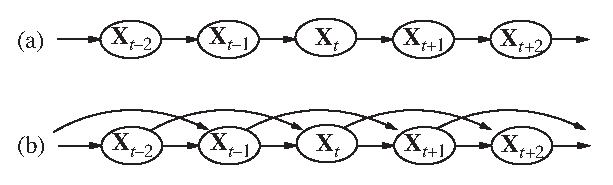
\includegraphics{Chapters/MultiAgentProbabilisticSearch/BayesianFiltering/Figs/markov-processes.eps}
    \caption{First (a) and second (b) order Markov processes \cite{AIAMA}}
    \label{fig:markov-processes}
\end{figure}
It also is possible to calculate the probability of the process experiencing a sequence of states from timesteps 1 as far as t, using the chain rule of probability and the Markov property:
$P(X_{1:t}) = P(X_1, X_2, ..., X_t) = P(X_1)\times P(X_2 | X_1)\times P(X_3 | X_2, X_1) \times P(X_t | X_{t-1}, X_{t-2}, ... , X_1) = P(X_1) \times \prod_{i=2}^{t}{P(X_i | x_{i-1})}$. Marginalization over variables in this sequence allows the calculation of many useful quantities.
\par

\subsubsection{HMM Description}
Hidden Markov Models (HMMs) are models that build on the Markov Process model, which describe the evolution of a random system in the language of probability theory. HMMs assume that the system being modeled can be described by a Markov process, but that the states of this process are unobservable. This means that it isn't possible to determine the state of the system exactly at any given point in time. However, it is possible to make an observation of a random variable that is related to the hidden state which yields information about the hidden state. This is visualised in Figure \ref{fig:hmm}
\begin{figure}[]
    \centering
    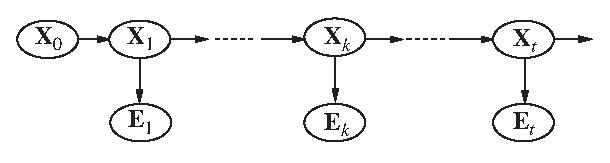
\includegraphics{Chapters/MultiAgentProbabilisticSearch/BayesianFiltering/Figs/smoothing-dbn.eps}
    \caption{A visualisation of a HMM \cite{AIAMA}}
    \label{fig:hmm}
\end{figure}
, where the Markov Process is shown by the variables $X_i$ and the observation variables are shown by variables $E_i$. A HMM can be specified by a triple, $\lambda$ = $(T, O, \pi)$, where $T$ is the stochastic transition matrix, $\pi$ is the initial distribution $P(X_1)$ and O describes the conditional probability of an observation given that the system is in a certain state: $O(E_i, X_i) = P(E_{i} | X_{i})$. Taken together, it is then possible to specify the joint distribution of the hidden state variables and the evidence variables, analogous to the Markov Process: 
$
P(X_{1:t}, E_{1:t}) = P(X_1, X_2, ..., X_t, E_1, E_2, ..., E_t) = P(X_1) \times P(E_1 | X_1) \times
\prod_{i=2}^{t}{(P(X_i | x_{i-1}) \times P(E_t | X_t))}.
$Given representation, it is then possible to answer questions such as:
\begin{itemize}
    \item Given the HMM, $\lambda$, determine the probability of occurrence of a particular observation sequence, $P(E_{1:t} | \lambda)$
    \item Given a sequence of observations $(E_1, E_2, ..., E_n)$, what is the most likely sequence of hidden states that led to these observations? i.e. find \[\argmax_{X_{1:t}} P(X_{1:t} | E_{1:t})\].
    \item Determine the parameters of $T$ and $O$, given a training set of observations, i.e. find the solution to \[\argmax_{\lambda} P(E_{1:t} | \lambda)\].
    \item Filtering: What is the current distribution of the hidden state given all previous evidence ('belief state') of the agent at time t: $P(X_t | E_{1:t})$?
    \item Prediction: What is the distribution of the hidden state in the future, given all evidence to date: $P(X_{t+k} | E_{1:t})$, for some k$>$0?
    \item Smoothing: What is the distribution of a past state given all observations up to the current point in time: $P(X_k | E_{1:t})$, for some 0 $\leq$ k $<$ t?
\end{itemize}
\par

%Might include a subsection on a taxonomy of commonly used HMMs.

\subsubsection{Summary}
In summary, HMMs can be used to abstractly describe the evolution of a stochastic system. They have been used to achieve state of the art performance in problems such as speech recognition \cite{ChiuSTATE-OF-THE-ARTMODELS} and ... . An comprehensive overview of extensions to the vanilla HMM can be found at \cite{Murphy1994DynamicLearning}.

\subsection{Dynamic Bayesian Networks}
\nomenclature[]{DBN}{Dynamic Bayesian Network}
\nomenclature[]{BN}{Bayesian Network}
\nomenclature[]{CPD}{Conditional Probability Distribution}
\placeholder{}
Dynamic Bayesian Networks are a generalization of HMMs and are used to model time series, without being limited to the assumptions of HMMs. The key difference between DBNs and HMMs are is that DBNs are not limited in how they decompose the state of a complex stochastic system into the variables that represent its constituent distributions\cite{AIAMA}. Technically, every DBN can be represented as a HMM and visa versa, however, the number of parameters that need to be detemined to represent DBNs can be significantly less that that of HMMs. This is a manifestation of how specifying a full joint discrete distribution can require an exponential number of probabilities, whereas specifying the same joint distribution as factored conditional distributions may require far fewer.

\subsubsection{A Note on Bayesian Networks}
A Bayesian Network (BN) is a graphical way to represent a particular factorization of a joint distribution. For a detailed explanation, the reader is referred to \cite{KollerPGM}. To fully explain a complex system, it is often natural to model it as the joint distribution of a number of random variables. This is in general intractable \cite{KollerPGM}. In order to circumvent this, independence properties in the distribution can be exploited to provide a much more compact representation of the distribution. BNs exploit the fact that independence is a strong notion that doesn't often occur in the real-world; however conditional independence is a weaker property that is far more prevalent, which still leads to the desired compact representation. BNs are described by a directed acyclic graph (DAG), $G$. The nodes in the graph correspond to the random variables whose joint distribution is of interest, and the arcs represent conditional independences. Specifically, if one Burglary points to Alarm as in figure \ref{BayesianNetwork}, it is implied that the distribution of Alarm is conditionally independent on all other nodes in the network given Burglary. This means that only local conditional probability distribution must be provided in order to specify the full joint distribution.

\begin{figure}
%example bayesian network figure
\begin{tikzpicture}[
  node distance=1cm and 0cm,
  mynode/.style={draw,ellipse,text width=2cm,align=center}
]
\node[mynode] (i) {Burglary};
\node[mynode,below right=of i] (g) {Alarm};
\node[mynode,above right=of g] (c) {Earthquake};
\path %(ra) edge[latex-] (sp)
(g) edge[latex-] (c) 
(g) edge[latex-] (i);
\node[left=0.5cm of i]
{
\begin{tabular}{cM{2}M{2}}
\toprule
\multicolumn{2}{c}{Burglary} \\
\multicolumn{1}{c}{T} & \multicolumn{1}{c}{F} \\
\cmidrule(r){1-2}
0.001 & 0.999 \\
\bottomrule
\end{tabular}
};
\node[right=0.5cm of c]
{
\begin{tabular}{cM{2}M{2}}
\toprule
\multicolumn{2}{c}{Earthquake} \\
\multicolumn{1}{c}{T} & \multicolumn{1}{c}{F} \\
\cmidrule(r){1-2}
0.008 & 0.992 \\
\bottomrule
\end{tabular}
};
\node[below=0.5cm of g]
{
\begin{tabular}{ccM{2}M{2}}
\toprule
& & \multicolumn{2}{c}{Alarm} \\
\multicolumn{2}{l}{Burglary Earthquake} & \multicolumn{1}{c}{T} & \multicolumn{1}{c}{F} \\
\cmidrule(r){1-2}\cmidrule(l){3-4}
F & F & 0.01 & 0.99 \\
F & T & 0.95 & 0.05 \\
T & F & 0.8 & 0.2 \\
T & T & 0.99 & 0.01 \\
\bottomrule
\end{tabular}
};
\end{tikzpicture}

\caption{Simple Bayesian Network based on \cite[P.~512]{AIAMA}}
\label{fig:BayesianNetwork}
\end{figure}











\subsubsection{Dynamic Bayesian Network Description}
A Dynamic Bayesian Network is a Bayesian Network that represents a general temporal probability model that describes a random system which is assumed to have a number of random variables, some of which are observable and some not. \cite{AIAMA}.

\subsubsection{Recursive State Estimation}


\subsubsection{}

\subsection{Filtering Algorithms}
\placeholder{}
This contains the details of Bayesian filtering algorithms.

\subsection{Prediction Algorithms}
\placeholder{}
This contains the details of prediction algorithms
%%%%%%%%%%%%%%%%%%%%%%%%%% Bayesian Filtering Sections %%%%%%%%%%%%%%%%%%%%%%%%%%



%%%%%%%%%%%%%%%%%%%%%%%%%% Search Termination Sections %%%%%%%%%%%%%%%%%%%%%%%%%%
\section{Search Termination Criteria}

\subsection{Heuristic Search Termination}
\subsection{Sequential Probability Ratio Test}
%%%%%%%%%%%%%%%%%%%%%%%%%% Search Termination Sections %%%%%%%%%%%%%%%%%%%%%%%%%%

%%%%%%%%%%%%%%%%%%%%%%%%%% Decision Theory %%%%%%%%%%%%%%%%%%%%%%%%%%
\section{Solving the Decision Problem}
\subsection{Decision Theory}

\subsection{Decision Strategies}

\subsection{Modular Pipeline}
Here is where a modular 

%%%%%%%%%%%%%%%%%%%%%%%%%% Decision Theory %%%%%%%%%%%%%%%%%%%%%%%%%%
\chapter{Simulation Environment}
\placeholder{}
%!TEX root = ../thesis.tex
%*******************************************************************************
%*********************************** First Chapter *****************************
%*******************************************************************************

\chapter{Conclusion}
At the beginning of this thesis, we identified two research questions: 
\begin{itemize}
    \item Can an agent-based software system be developed to run on a system of heterogeneous autonomous aerial vehicles to aid the tasks of scene surveying and target localisation in a hazardous environment?  
    \item Can a high-fidelity simulation environment be created,
%to simulate a hazardous environment
which can generate realistic salient data to support the process of prototyping AI systems designed to aid the management of real-world hazardous scenarios?
\end{itemize}
These were identified based on the ROCSAFE project and we aimed to find answers to them with the work done as part of this thesis.

\par The second question was addressed in Chapter \ref{chap:HighFidelitySim}, where we provided the details of a custom-built high-fidelity simulation environment using the UE4 game engine. We identified realistic data that was relevant to hazardous real-world scenarios, which included images taken from the perspective of a RAV and CBRN sensor data. We simulated this data through the use of tools that are part of UE4 as well as the use of the Airsim \cite{Shah2017AirSim:Vehicles} plugin for UE4. This aided the tasks of developing techniques to solve the problem scene surveying and target localisation, identified in the second research questions, by ensuring that the developed methods could be tested at low cost and high speed.

\par We can also answer the first research question positively, based on the the work outlined in Chapters \ref{chapter:SceneSurveying} and \ref{chap:targetLocalisation}. We developed a software system that built on previous related work which was highly modular and could be calibrated to reflect realistic varying parameters among aerial vehicles, such as operational speed. The task of scene surveying was addressed in Chapter \ref{chapter:SceneSurveying} and we devised a method of discretising the region to be surveyed along with algorithms that would set out routes for the aerial vehicles. We tested this using our developed high-fidelity simulation environment, which closely mirrored intended real-world usage. The task of target localisation was tackled in Chapter \ref{chap:targetLocalisation}. We provided the details of a system that could use multiple RAVs to effectively find the hidden location of one or more targets, based on sensor data. We used the Sequential Probability Ratio Test as a cutoff criterion for the search termination. We implemented a number of sampling strategies and investigated the effects of varying key parameters in the search, such as the prior distribution and the number of targets present. The results indicate that for "reasonable" choices of these parameters, the search could localise one or more targets according to the error rates set out by the SPRT.
%\include{Chapter7/chapter7}



% ********************************** Back Matter *******************************
% Backmatter should be commented out, if you are using appendices after References
%\backmatter

% ********************************** Bibliography ******************************
\begin{spacing}{0.9}

% To use the conventional natbib style referencing
% Bibliography style previews: http://nodonn.tipido.net/bibstyle.php
% Reference styles: http://sites.stat.psu.edu/~surajit/present/bib.htm

\bibliographystyle{apalike}
%\bibliographystyle{unsrt} % Use for unsorted references  
%\bibliographystyle{plainnat} % use this to have URLs listed in References
\cleardoublepage
\bibliography{References/references} % Path to your References.bib file


% If you would like to use BibLaTeX for your references, pass `custombib' as
% an option in the document class. The location of 'reference.bib' should be
% specified in the preamble.tex file in the custombib section.
% Comment out the lines related to natbib above and uncomment the following line.

%\printbibliography[heading=bibintoc, title={References}]


\end{spacing}

% ********************************** Appendices ********************************

\begin{appendices} % Using appendices environment for more functunality

%!TEX root = ../thesis.tex
% ******************************* Thesis Appendix A ****************************
\chapter{How to install \LaTeX} 

\section*{Windows OS}

\subsection*{TeXLive package - full version}
\begin{enumerate}
\item	Download the TeXLive ISO (2.2GB) from\\
\href{https://www.tug.org/texlive/}{https://www.tug.org/texlive/}
\item	Download WinCDEmu (if you don't have a virtual drive) from \\
\href{http://wincdemu.sysprogs.org/download/}
{http://wincdemu.sysprogs.org/download/}
\item	To install Windows CD Emulator follow the instructions at\\
\href{http://wincdemu.sysprogs.org/tutorials/install/}
{http://wincdemu.sysprogs.org/tutorials/install/}
\item	Right click the iso and mount it using the WinCDEmu as shown in \\
\href{http://wincdemu.sysprogs.org/tutorials/mount/}{
http://wincdemu.sysprogs.org/tutorials/mount/}
\item	Open your virtual drive and run setup.pl
\end{enumerate}

or

\subsection*{Basic MikTeX - \TeX~ distribution}
\begin{enumerate}
\item	Download Basic-MiK\TeX (32bit or 64bit) from\\
\href{http://miktex.org/download}{http://miktex.org/download}
\item	Run the installer 
\item	To add a new package go to Start >> All Programs >> MikTex >> Maintenance (Admin) and choose Package Manager
\item	Select or search for packages to install
\end{enumerate}

\subsection*{TexStudio - \TeX~ editor}
\begin{enumerate}
\item	Download TexStudio from\\
\href{http://texstudio.sourceforge.net/\#downloads}
{http://texstudio.sourceforge.net/\#downloads} 
\item	Run the installer
\end{enumerate}

\section*{Mac OS X}
\subsection*{MacTeX - \TeX~ distribution}
\begin{enumerate}
\item	Download the file from\\
\href{https://www.tug.org/mactex/}{https://www.tug.org/mactex/}
\item	Extract and double click to run the installer. It does the entire configuration, sit back and relax.
\end{enumerate}

\subsection*{TexStudio - \TeX~ editor}
\begin{enumerate}
\item	Download TexStudio from\\
\href{http://texstudio.sourceforge.net/\#downloads}
{http://texstudio.sourceforge.net/\#downloads} 
\item	Extract and Start
\end{enumerate}


\section*{Unix/Linux}
\subsection*{TeXLive - \TeX~ distribution}
\subsubsection*{Getting the distribution:}
\begin{enumerate}
\item	TexLive can be downloaded from\\
\href{http://www.tug.org/texlive/acquire-netinstall.html}
{http://www.tug.org/texlive/acquire-netinstall.html}.
\item	TexLive is provided by most operating system you can use (rpm,apt-get or yum) to get TexLive distributions
\end{enumerate}

\subsubsection*{Installation}
\begin{enumerate}
\item	Mount the ISO file in the mnt directory
\begin{verbatim}
mount -t iso9660 -o ro,loop,noauto /your/texlive####.iso /mnt
\end{verbatim}

\item	Install wget on your OS (use rpm, apt-get or yum install)
\item	Run the installer script install-tl.
\begin{verbatim}
	cd /your/download/directory
	./install-tl
\end{verbatim}
\item	Enter command `i' for installation

\item	Post-Installation configuration:\\
\href{http://www.tug.org/texlive/doc/texlive-en/texlive-en.html\#x1-320003.4.1}
{http://www.tug.org/texlive/doc/texlive-en/texlive-en.html\#x1-320003.4.1} 
\item	Set the path for the directory of TexLive binaries in your .bashrc file
\end{enumerate}

\subsubsection*{For 32bit OS}
For Bourne-compatible shells such as bash, and using Intel x86 GNU/Linux and a default directory setup as an example, the file to edit might be \begin{verbatim}
edit $~/.bashrc file and add following lines
PATH=/usr/local/texlive/2011/bin/i386-linux:$PATH; 
export PATH 
MANPATH=/usr/local/texlive/2011/texmf/doc/man:$MANPATH;
export MANPATH 
INFOPATH=/usr/local/texlive/2011/texmf/doc/info:$INFOPATH;
export INFOPATH
\end{verbatim}
\subsubsection*{For 64bit OS}
\begin{verbatim}
edit $~/.bashrc file and add following lines
PATH=/usr/local/texlive/2011/bin/x86_64-linux:$PATH;
export PATH 
MANPATH=/usr/local/texlive/2011/texmf/doc/man:$MANPATH;
export MANPATH 
INFOPATH=/usr/local/texlive/2011/texmf/doc/info:$INFOPATH;
export INFOPATH

\end{verbatim}



%\subsection{Installing directly using Linux packages} 
\subsubsection*{Fedora/RedHat/CentOS:}
\begin{verbatim} 
sudo yum install texlive 
sudo yum install psutils 
\end{verbatim}


\subsubsection*{SUSE:}
\begin{verbatim}
sudo zypper install texlive
\end{verbatim}


\subsubsection*{Debian/Ubuntu:}
\begin{verbatim} 
sudo apt-get install texlive texlive-latex-extra 
sudo apt-get install psutils
\end{verbatim}

%!TEX root = ../thesis.tex
% ******************************* Thesis Appendix B ********************************

\chapter{Histograms of Time To Decision}



\begin{landscape}
\centering
\vspace*{\fill}
\begin{table}[h!]
  \centering
  \begin{tabular}{ | c | c | c | c | c |}
    \hline
    & $\epsilon$-Greedy & Sweep & Random & Saccadic \\
    %\hline
    % \multicolumn{2}{c}{Initial Uniform Distribution of Belief Over Grid Cells}\\
    %\hline
    %single UAV
    %\begin{minipage}[c][height][c]{width}
    Gaussian & \vline
    \begin{minipage}[c][36mm][c]{38mm}
      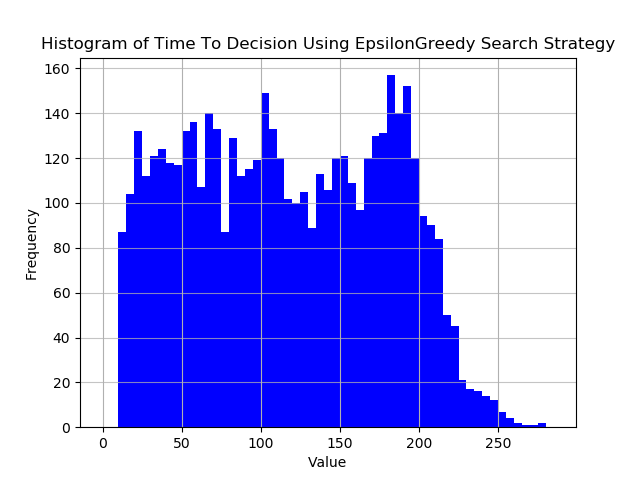
\includegraphics[width=38mm, height=38mm]{Chapters/MultiAgentTargetDetection/Figs/Results/Prior/Gaussian/SingleAgentSingleSourceGaussianEpsilonGreedyHistogram.png}
    \end{minipage}
    &
    %\hline
    %\multicolumn{2}{c}{Initial Discretised Gaussian Distribution of Belief Over Grid Cells (random mean, covariance matrix = [[], []]}\\
    %\hline
    %single UAV
    %\begin{minipage}[c][height][c]{width}
    \begin{minipage}[c][36mm][c]{38mm}
      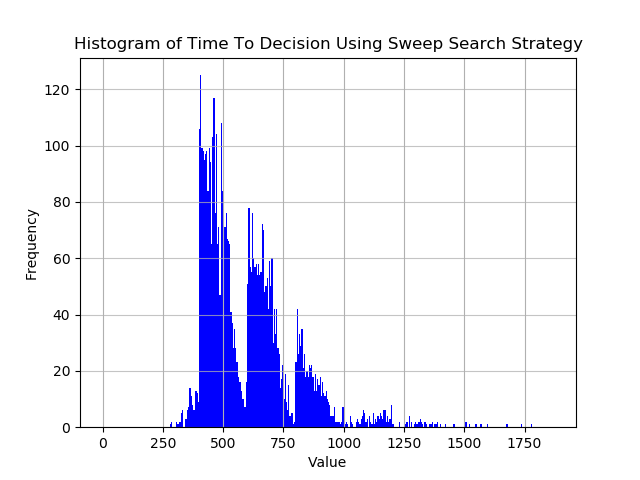
\includegraphics[width=38mm, height=38mm]{Chapters/MultiAgentTargetDetection/Figs/Results/Prior/Gaussian/SingleAgentSingleSourceGaussianSweepHistogram.png}

    \end{minipage}
    &
    \begin{minipage}[c][36mm][c]{38mm}
      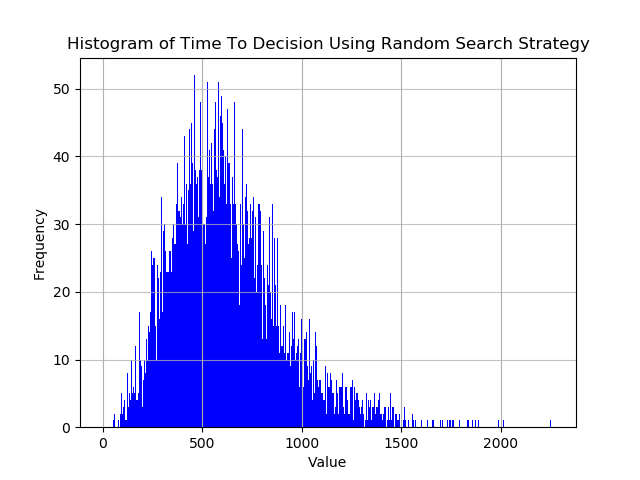
\includegraphics[width=38mm, height=38mm]{Chapters/MultiAgentTargetDetection/Figs/Results/Prior/Gaussian/SingleAgentSingleSourceGaussianRandomHistogram.png}
    \end{minipage}
    &
    \begin{minipage}[c][36mm][c]{38mm}
      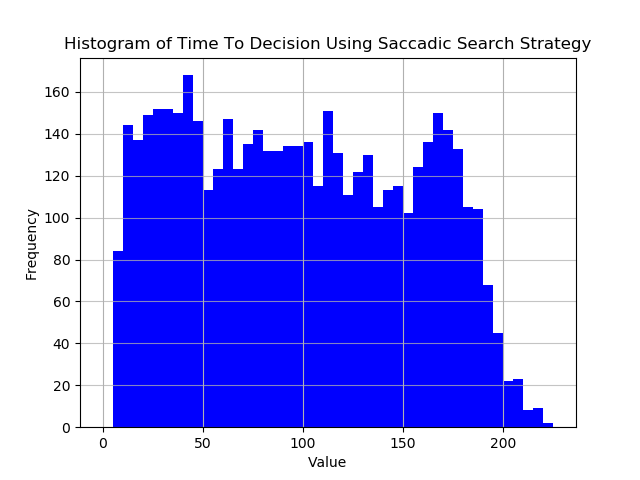
\includegraphics[width=38mm, height=38mm]{Chapters/MultiAgentTargetDetection/Figs/Results/Prior/Gaussian/SingleAgentSingleSourceGaussianSaccadicHistogram.png}
    \end{minipage}
    \\
    %&
    %\small
    %\begin{tabular}{c|c|c|c|c|c|c|c}
    %    Strategy & p(T \Romannum{1}) & p(T \Romannum{2}) & Sim. FPR & Sim. FNR & E[TTD] & Prec. & Rec \\
    %    \hline
    %    $\epsilon$ -Greedy& 4 & 2 & 0.05 & 233.2 & 2303.3 & 2 & 9\\
    %    Sweep & 4 & 2 & 0.05 & 233.2 & 2303.3 & 2 & 9\\
    %    Saccadic & 4 & 2 & 0.05 & 233.2 & 2303.3 & 2 & 9\\
    %    Random & 4 & 2 & 0.05 & 233.2 & 2303.3 & 2 & 9\\

    %\end{tabular}
    %\normalsize

    \hline
   
  \end{tabular}
  \caption{Results of running the target localisation simulation with a  uniform initial belief distribution and Gaussian initial belief distribution. p(T \Romannum{1}) = The probability of making a type \Romannum{1} error using the SPRT, p(T \Romannum{2}) = The probability of making a type \Romannum{1} error using the SPRT, Sim. FPR = The simulated false positive rate of the sensor, Sim. FNR = The simulated false negative rate of the sensor, E[TTD] = The expected amount of timesteps until a decision is made, Prec. = precision, Rec. = Recall. }\label{table:ORToolsResults}
\end{table}
\end{landscape}


\end{appendices}

% *************************************** Index ********************************
\printthesisindex % If index is present

\end{document}
